% InteriorPoint_QP_beamer.tex
% 5-slide Beamer presentation explaining interior-point techniques for a convex quadratic program.
% Includes illustration with the optimal point on the boundary.

\documentclass{beamer}
\usetheme{default}
\usepackage{amsmath,amsfonts,amssymb}
\usepackage{tikz}
\usepackage{pgfplots}
\pgfplotsset{compat=1.18}
\setbeamertemplate{navigation symbols}{}
\title{Interior-point techniques for a quadratic program}
\author{Prepared by ChatGPT}
\date{\today}

\begin{document}
\begin{frame}
  \titlepage
\end{frame}

% Slide 1: Problem statement + KKT
\begin{frame}{Convex quadratic program: problem and optimality}
\vspace{-2mm}
Consider the convex quadratic program in standard form:
\begin{align*}
  &\min_{x\in\mathbb{R}^n} \; f(x) := \tfrac{1}{2}x^T Q x + c^T x\\
  &\text{subject to }\; A x = b, \quad x \ge 0,
\end{align*}
where $Q\succeq 0$, $A\in\mathbb{R}^{m\times n}$.

First-order (KKT) conditions (existence of multipliers $y,z$):
\begin{align*}
  Qx + c + A^T y - z &= 0 \quad (\text{stationarity})\\
  Ax - b &= 0 \quad (\text{primal feasibility})\\
  X Z e &= 0,\quad x\ge0,\ z\ge0 \quad(\text{complementarity})
\end{align*}
where $X=\mathrm{diag}(x)$, $Z=\mathrm{diag}(z)$, $e$ is the vector of ones.

\vspace{2mm}
Interior-point idea: enforce strict positivity $x>0, z>0$ and drive $XZe=\mu e$ to zero along the \emph{central path} as $\mu\downarrow0$.
\end{frame}

% Slide 2: Full Newton system (x, y, z)
\begin{frame}{Full Newton step for primal--dual system}
The perturbed KKT conditions for $\mu>0$ are:
\begin{align*}
  Qx + c + A^T y - z &= 0, \\
  Ax - b &= 0, \\
  XZe &= \mu e.
\end{align*}
We linearize these equations at $(x,y,z)$ to get the Newton system for $(\Delta x, \Delta y, \Delta z)$:
\[
  \begin{bmatrix}
    Q & A^T & -I \\
    A & 0   & 0   \\
    Z & 0   & X
  \end{bmatrix}
  \begin{bmatrix}
    \Delta x \\
    \Delta y \\
    \Delta z
  \end{bmatrix}
  = -\begin{bmatrix}
    r_d \\
    r_p \\
    r_c
  \end{bmatrix},
\]
where
\begin{align*}
  r_d &= Qx + c + A^T y - z,\\
  r_p &= Ax - b,\\
  r_c &= XZe - \mu e.
\end{align*}
This 3-block structure is the foundation of primal--dual interior-point methods.
\end{frame}

% Slide 3: Central path illustration (interior optimum)
\begin{frame}{Illustration of the central path}
\textbf{Definition:} The \emph{central path} is the trajectory of strictly feasible points $(x(\mu), y(\mu), z(\mu))$ satisfying
\[
Qx(\mu) + c + A^T y(\mu) - z(\mu) = 0, \quad Ax(\mu) = b, \quad X(\mu) Z(\mu)e = \mu e,\; \mu>0.
\]
As $\mu \to 0$, the path converges to the optimal solution $(x^*,y^*,z^*)$.

\vspace{2mm}
\textbf{Geometric intuition:}
\begin{itemize}
  \item Each $\mu$ defines a barrier problem that smooths the feasible region.
  \item The central path traces the minimizers of these smoothed problems.
  \item Interior-point methods follow this path using Newton directions.
\end{itemize}

\vspace{2mm}
\begin{center}
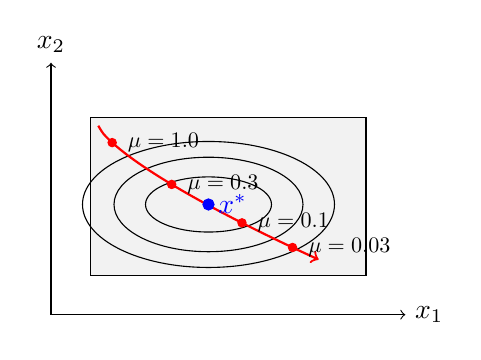
\begin{tikzpicture}[scale=1]
  \draw[->] (0,0) -- (4.5,0) node[right] {$x_1$};
  \draw[->] (0,0) -- (0,3.2) node[above] {$x_2$};
  \draw[fill=gray!10] (0.5,0.5) -- (4,0.5) -- (4,2.5) -- (0.5,2.5) -- cycle;
  \draw (2,1.4) ellipse (1.6 and 0.8);
  \draw (2,1.4) ellipse (1.2 and 0.6);
  \draw (2,1.4) ellipse (0.8 and 0.35);
  \draw[thick,red,->] plot [smooth,domain=0:1] ( {0.6+2.8*\x^1.2}, {2.4-1.7*\x^0.9} );
  \foreach \m/\t in {1.0/0.1,0.3/0.4,0.1/0.7,0.03/0.9}{
    \filldraw[red] ({0.6+2.8*\t^1.2},{2.4-1.7*\t^0.9}) circle (1.5pt);
    \node[anchor=west,scale=0.8] at ({0.6+2.8*\t^1.2+0.1},{2.4-1.7*\t^0.9}) {$\mu=\m$};}
  \filldraw[blue] (2,1.4) circle (2pt) node[right] {$x^*$};
\end{tikzpicture}
\end{center}
\end{frame}

% Slide 4: Central path with boundary optimum
\begin{frame}{Central path ending at a boundary optimum}
In many convex QPs, the optimal solution lies on the \textbf{boundary} of the feasible region. The central path still approaches this point smoothly from the interior.

\vspace{2mm}
\textbf{Example illustration:}
\begin{center}
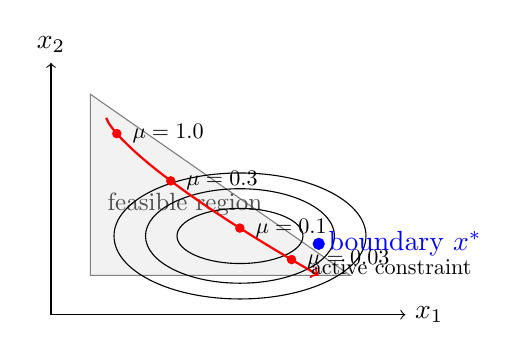
\begin{tikzpicture}[scale=1]
  % Axes
  \draw[->] (0,0) -- (4.5,0) node[right] {$x_1$};
  \draw[->] (0,0) -- (0,3.2) node[above] {$x_2$};
  % Feasible region (triangle)
  \filldraw[fill=gray!10,draw=gray] (0.5,0.5) -- (3.8,0.5) -- (0.5,2.8) -- cycle;
  \node[gray!60!black,scale=0.9] at (1.7,1.4) {feasible region};
  % Objective contours
  \draw (2.4,1.0) ellipse (1.6 and 0.8);
  \draw (2.4,1.0) ellipse (1.2 and 0.6);
  \draw (2.4,1.0) ellipse (0.8 and 0.35);
  % Central path (red curve approaching boundary)
  \draw[thick,red,->] plot [smooth,domain=0:1] ( {0.7+2.7*\x^1.3}, {2.5-2.0*\x^1.0} );
  % Markers for mu values
  \foreach \m/\t in {1.0/0.1,0.3/0.4,0.1/0.7,0.03/0.9}{
    \filldraw[red] ({0.7+2.7*\t^1.3},{2.5-2.0*\t^1.0}) circle (1.5pt);
    \node[anchor=west,scale=0.8] at ({0.7+2.7*\t^1.3+0.1},{2.5-2.0*\t^1.0}) {$\mu=\m$};}
  % Boundary optimum
  \filldraw[blue] (3.4,0.9) circle (2pt) node[right] {boundary $x^*$};
  % Boundary line label
  \node[rotate=0,anchor=west,scale=0.8] at (3.2,0.6) {active constraint};
\end{tikzpicture}
\end{center}

\vspace{2mm}
\textbf{Interpretation:} Even when $x^*$ is on the boundary, the central path remains strictly interior ($x>0$) for all $\mu>0$ and converges tangentially to the active constraint.
\end{frame}

% Slide 5: Primal-dual IPM
\begin{frame}{Primal--dual interior-point method \& practical notes}
Primal--dual methods work with both primal and dual variables and maintain perturbed complementarity:
\[XZ e = \sigma \mu e,\quad \mu=\frac{x^T z}{n},\quad 0<\sigma\le1.
\]
A common predictor--corrector algorithm (Mehrotra) computes a predictor (affine-scaling) step, estimates a \(\sigma\), then corrects to stay close to the central path.

Key practical points:
\begin{itemize}
  \item Use sparse symmetric linear algebra to solve the Newton/KKT system efficiently.
  \item Choose step-lengths to keep iterates positive; use Mehrotra predictor-corrector for fast practical convergence.
  \item Convergence: polynomial worst-case complexity (typically 30--60 iterations for large QPs in practice).
\end{itemize}

\vspace{2mm}
\textbf{Schematic: residual norms vs iterations}
\begin{center}
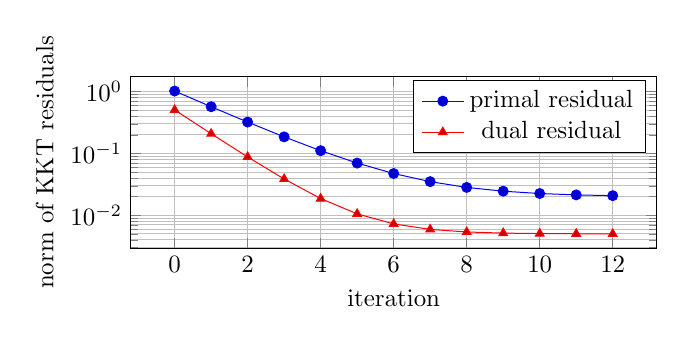
\begin{tikzpicture}[scale=0.9]
  \begin{axis}[width=9cm,height=4cm,xlabel=iteration,ylabel=norm of KKT residuals,ymode=log,grid=both]
    \addplot+[mark=*,domain=0:12,samples=13] (x,{exp(-0.6*x)+0.02});
    \addplot+[mark=triangle*,domain=0:12,samples=13] (x,{0.5*exp(-0.9*x)+0.005});
    \legend{primal residual,dual residual}
  \end{axis}
\end{tikzpicture}
\end{center}
\end{frame}

\end{document}
